\documentclass[12pt, a4paper, twoside]{article}

%% Preamble
\usepackage{pdfpages}           % Para incluir PDFs
\usepackage{graphicx}           % Para gráficos
\usepackage{subfiles}           % Para manejar subarchivos
\usepackage{hyperref}           % Para enlaces
\usepackage{listings}           % Para código fuente (ajusta lenguaje)
\usepackage[backend=biber]{biblatex}  % Para bibliografía
\usepackage{geometry}           % Para ajustar márgenes

% Ajustes de márgenes
\geometry{
	left=3cm,       % Margen izquierdo
	right=3cm,      % Margen derecho
	top=2.5cm,      % Margen superior
	bottom=2.5cm,   % Margen inferior
	headheight=15pt, % Altura del encabezado
	twoside          % Para documentos a dos caras
}

\addbibresource{references.bib}  % Archivo de bibliografía
\graphicspath{{images/}{../images/}} % Ruta para imágenes

\begin{document}
	
	%% Cover
	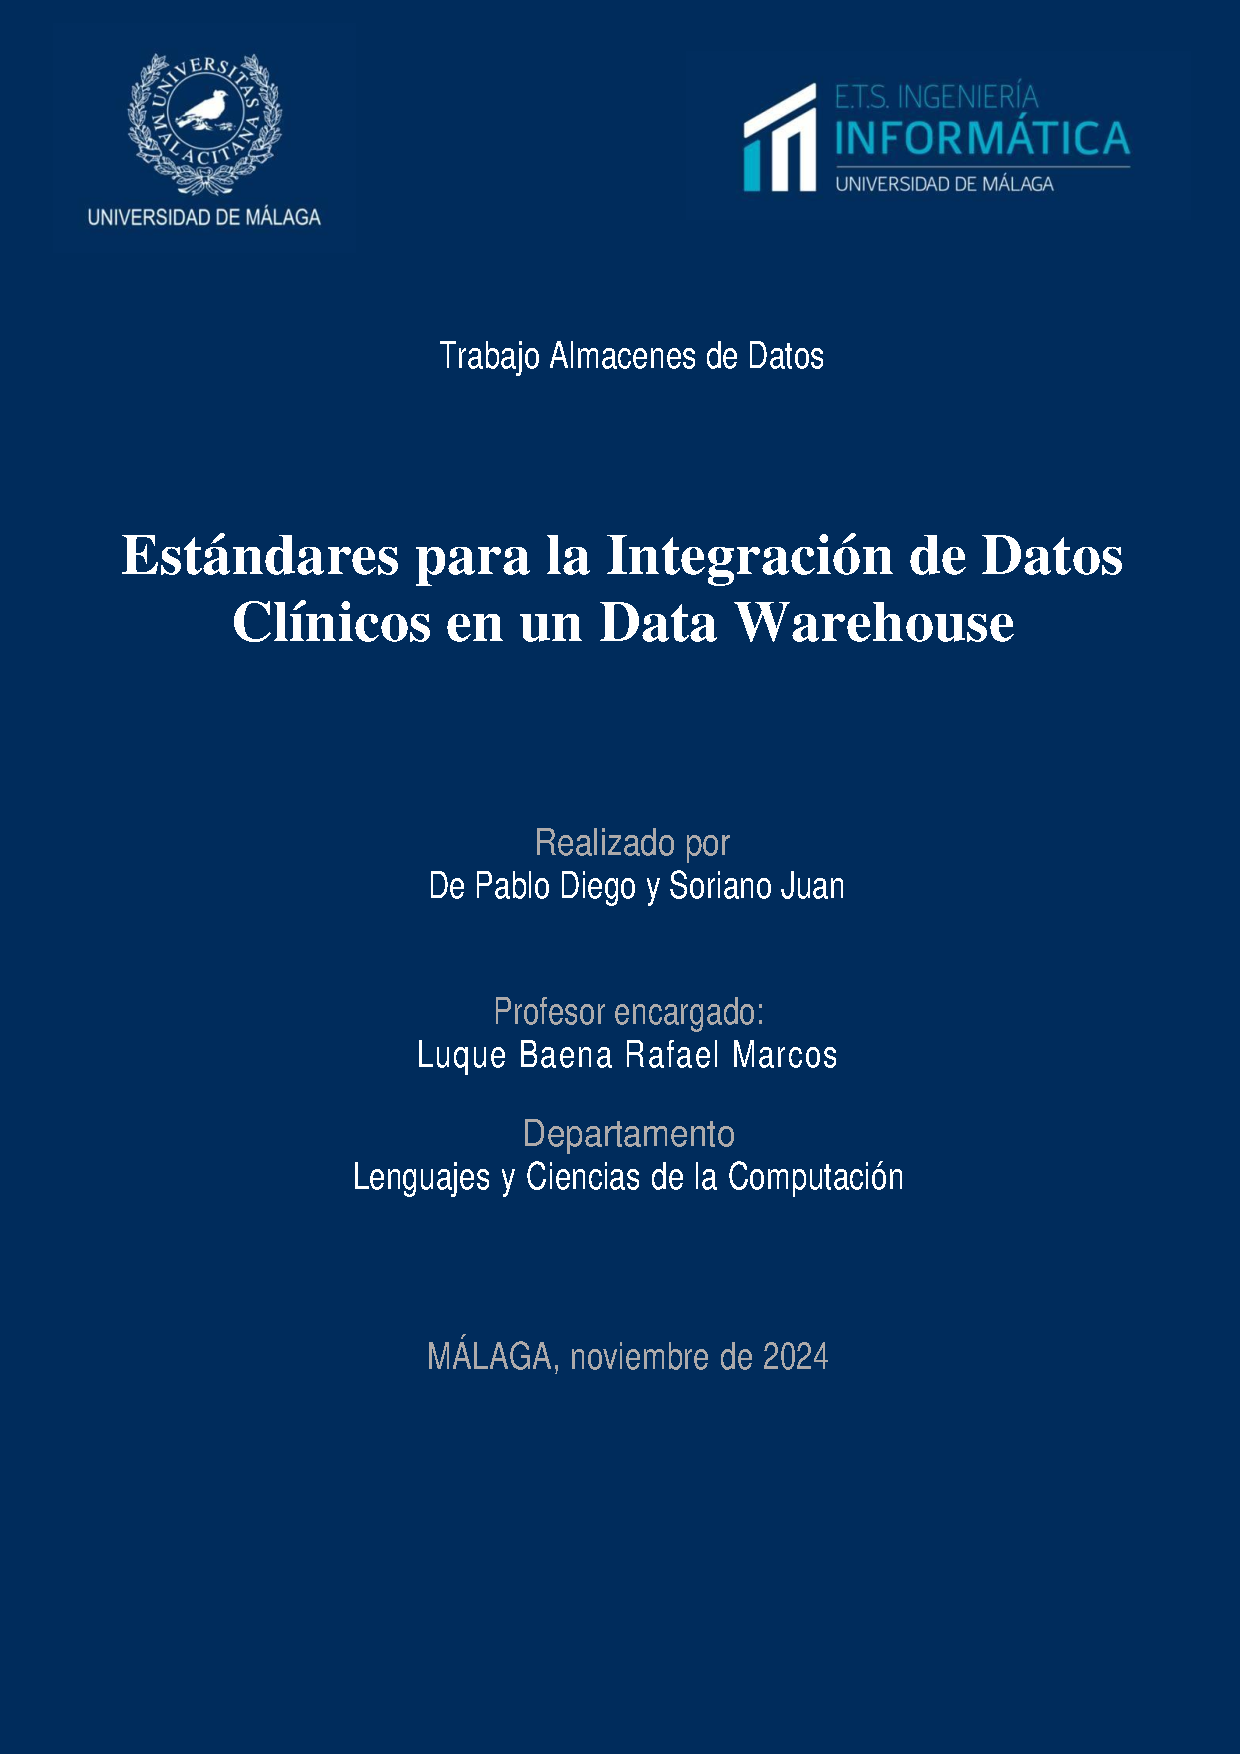
\includepdf[noautoscale=true, width=\paperwidth]{cover.pdf}
	
	%% Title
	\clearpage
	\setcounter{page}{1}
	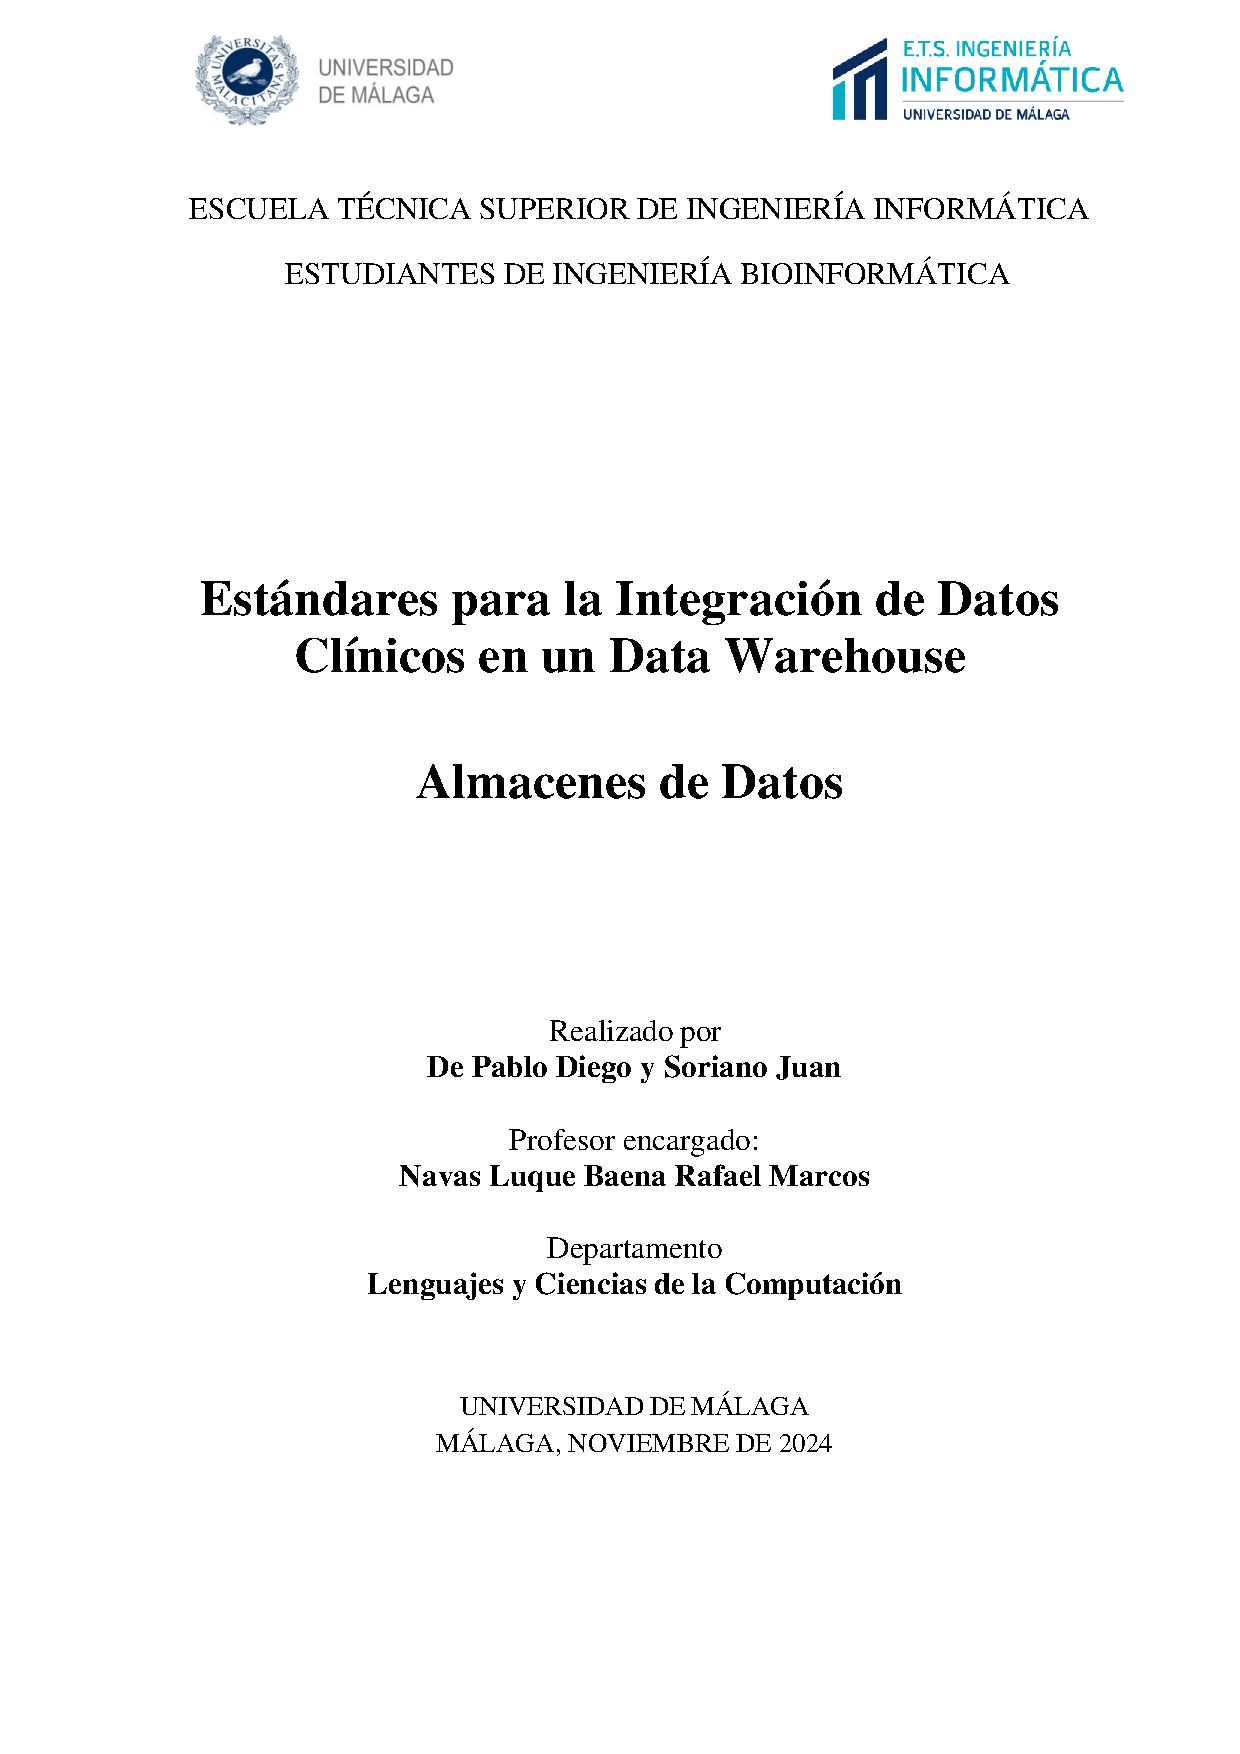
\includepdf[noautoscale=true, width=\paperwidth]{title.pdf}
	
	%%%%%%%%%%%%%%%%%%%%%%%%%%%%%%%%%%%%%%%%%%%%%%%%%%%%%%%%%%%%%%%%%%%%%%%%%%%
	
	% Índice automático
	\tableofcontents
	\newpage
	
	% Sections
	\section{Introducción a la Integración de Datos Clínicos en un Data Warehouse}
	Describe el propósito y la importancia de la integración de datos clínicos en un contexto centralizado.
	
	\section{Fundamentos y Conceptos Clave de los Data Warehouses en el Ámbito Clínico}
	Explica qué es un data warehouse, su estructura general y su relevancia en el manejo de datos de salud.
	
	\section{Estándares de Interoperabilidad en Datos Clínicos}
	Detalla los principales estándares (HL7, FHIR, SNOMED CT, LOINC) y cómo facilitan la integración y el intercambio de datos clínicos entre sistemas.
	
	\section{Arquitectura del Data Warehouse Clínico}
	Describe la arquitectura y los componentes de un data warehouse clínico, incluyendo las capas de almacenamiento, procesamiento y accesibilidad de los datos.
	
	\section{Proceso ETL para la Integración de Datos Clínicos}
	Explica las etapas de Extracción, Transformación y Carga (ETL) para normalizar y consolidar datos clínicos de diversas fuentes.
	
	\section{Beneficios de la Integración de Datos Clínicos}
	Enumera y detalla los beneficios clave de un data warehouse clínico: mejora en la toma de decisiones, apoyo a la investigación, análisis predictivo, etc.
	
	\section{Relación con el Curso de Almacenes de Datos}
	Analiza cómo los conceptos de la asignatura, como modelado de datos, arquitecturas de data warehouse y técnicas de ETL, se aplican en el desarrollo de un data warehouse clínico.
	
	\section{Ejemplos de Uso y Casos Prácticos de Integración de Datos Clínicos}
	Proporciona ejemplos de aplicación práctica, simulando la integración de datos de un sistema de EHR en un data warehouse usando algún estándar.
	
	\section{Conclusiones y Perspectivas Futuras en la Integración de Datos Clínicos}
	Ofrece un resumen de los puntos más importantes y discute posibles desarrollos futuros en la interoperabilidad y los data warehouses clínicos.
	
	%%%%%%%%%%%%%%%%%%%%%%%%%%%%%%%%%%%%%%%%%%%%%%%%%%%%%%%%%%%%%%%%%%%%%%%%%%%
	%% Back Cover
	
\includepdf[noautoscale=true, width=\paperwidth]{backcover.pdf}
	
\end{document}
